\documentclass{standalone}
\usepackage{tikz}
\usetikzlibrary{patterns, positioning}
\usepackage[sfdefault]{ClearSans} %% option 'sfdefault' activates Clear Sans as the default text font
\usepackage[T1]{fontenc}

\begin{document}
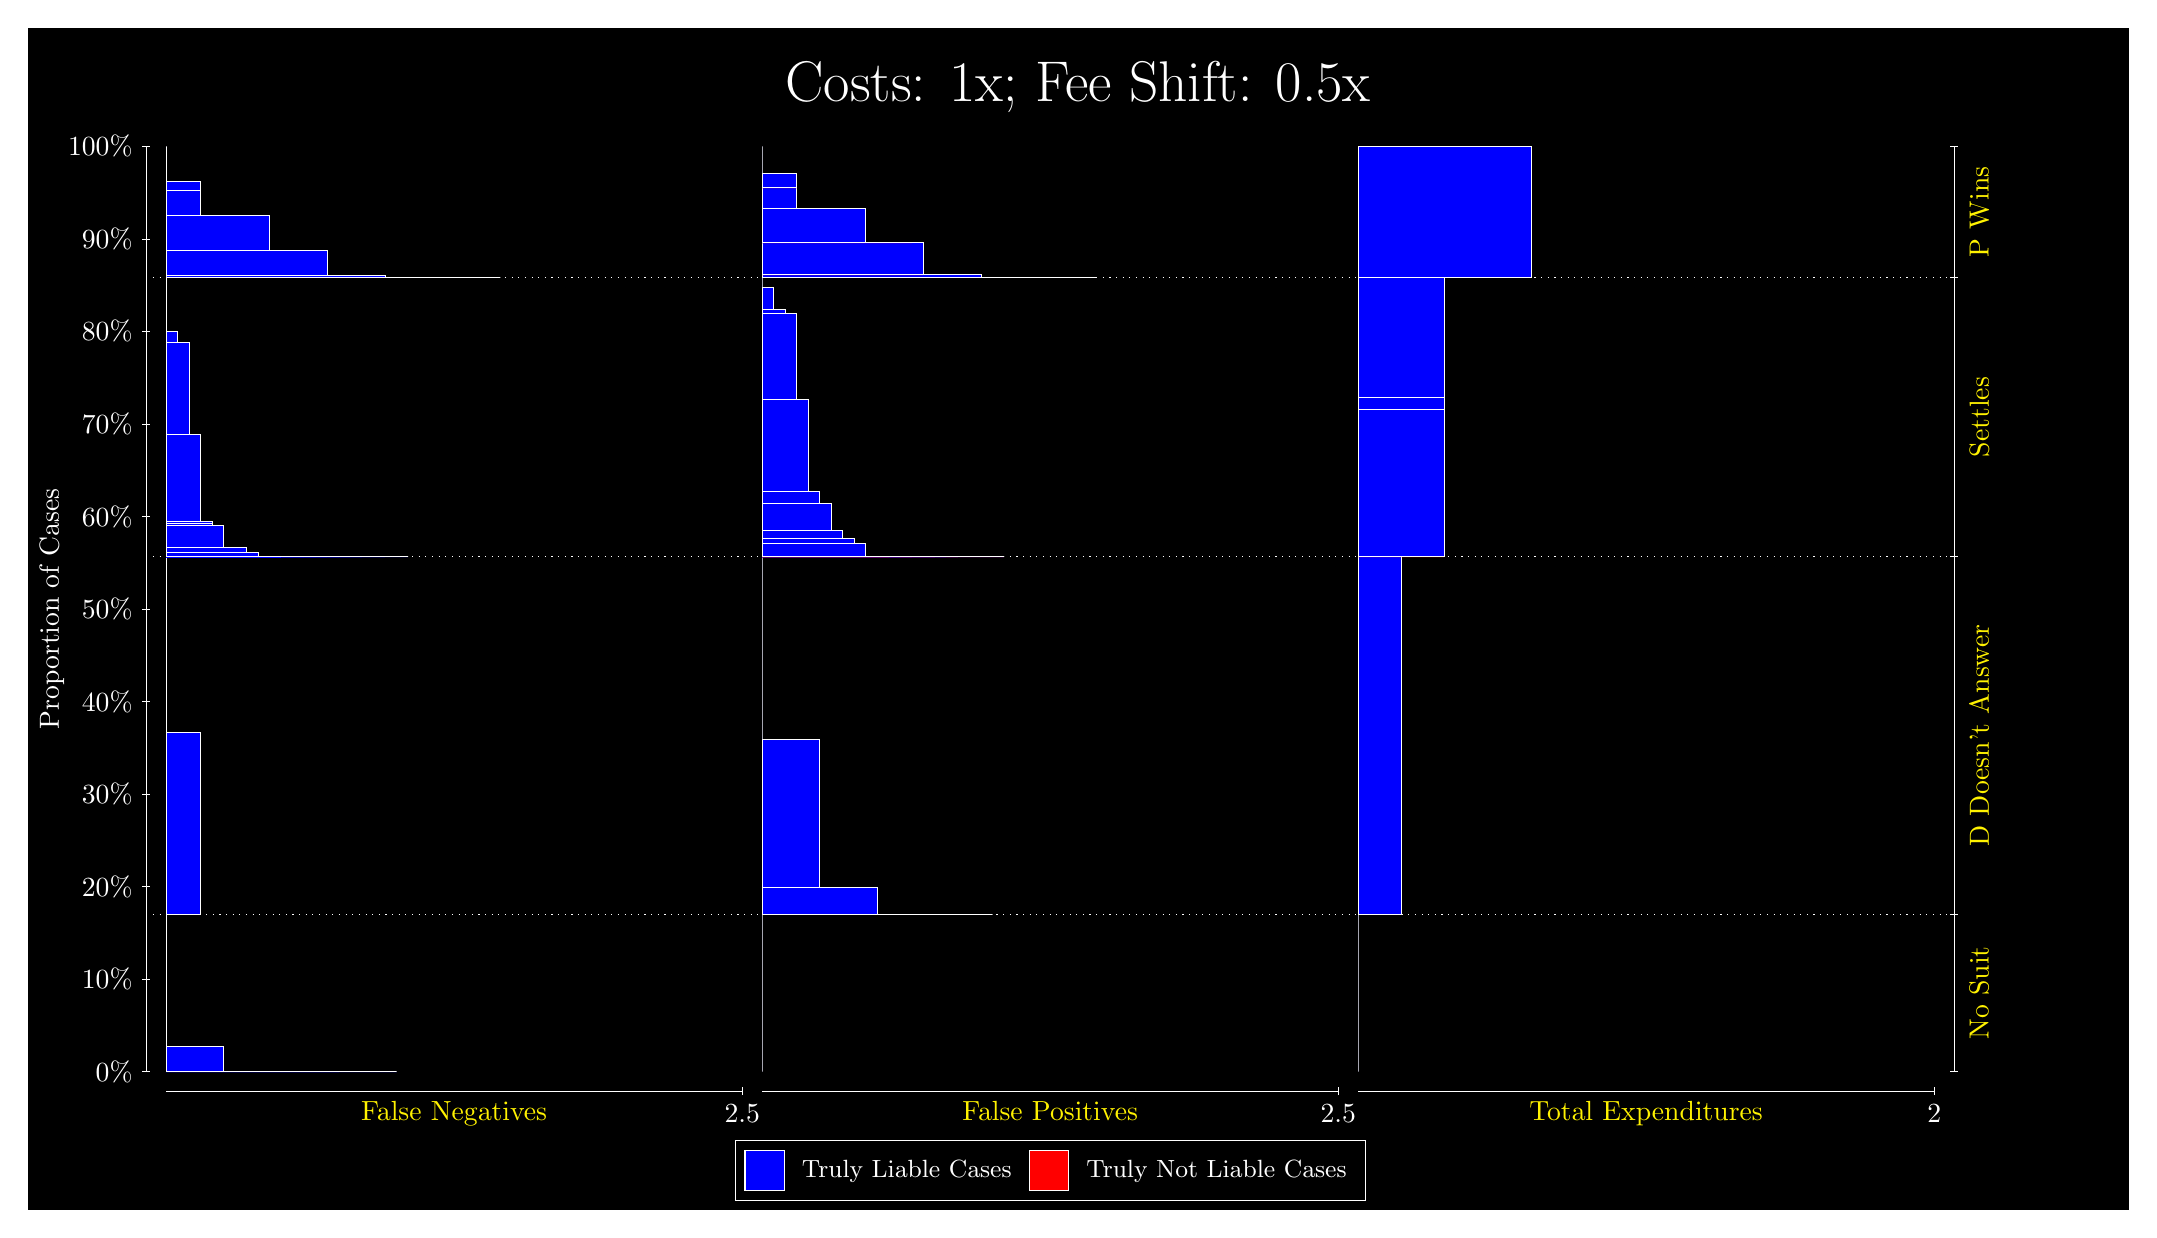
\begin{tikzpicture}
\draw[fill=black] (0,0) rectangle (26.667,15);
\draw[text=white] (0,13.5) rectangle (26.667,15) node[midway] {\huge Costs: 1x; Fee Shift: 0.5x};
\draw[white, very thin] (1.5,1.75) -- (1.5,13.5);
\node[rotate=90, text=white, anchor=center] at (0.3, 7.625) {Proportion of Cases};
\draw[white, very thin] (1.45,1.75) -- (1.55,1.75);
\node[text=white, anchor=east] at (1.45, 1.75) {0\%};
\draw[white, very thin] (1.45,2.925) -- (1.55,2.925);
\node[text=white, anchor=east] at (1.45, 2.925) {10\%};
\draw[white, very thin] (1.45,4.1) -- (1.55,4.1);
\node[text=white, anchor=east] at (1.45, 4.1) {20\%};
\draw[white, very thin] (1.45,5.275) -- (1.55,5.275);
\node[text=white, anchor=east] at (1.45, 5.275) {30\%};
\draw[white, very thin] (1.45,6.45) -- (1.55,6.45);
\node[text=white, anchor=east] at (1.45, 6.45) {40\%};
\draw[white, very thin] (1.45,7.625) -- (1.55,7.625);
\node[text=white, anchor=east] at (1.45, 7.625) {50\%};
\draw[white, very thin] (1.45,8.8) -- (1.55,8.8);
\node[text=white, anchor=east] at (1.45, 8.8) {60\%};
\draw[white, very thin] (1.45,9.975) -- (1.55,9.975);
\node[text=white, anchor=east] at (1.45, 9.975) {70\%};
\draw[white, very thin] (1.45,11.15) -- (1.55,11.15);
\node[text=white, anchor=east] at (1.45, 11.15) {80\%};
\draw[white, very thin] (1.45,12.325) -- (1.55,12.325);
\node[text=white, anchor=east] at (1.45, 12.325) {90\%};
\draw[white, very thin] (1.45,13.5) -- (1.55,13.5);
\node[text=white, anchor=east] at (1.45, 13.5) {100\%};

\draw[white, very thin] (24.457,1.75) -- (24.457,13.5);
\draw[white, very thin] (24.407,1.75) -- (24.507,1.75);
\node[anchor=west] at (24.407, 1.75) {};
\draw[white, very thin] (24.407,3.745) -- (24.507,3.745);
\node[anchor=west] at (24.407, 3.745) {};
\draw[white, very thin] (24.407,8.2876) -- (24.507,8.2876);
\node[anchor=west] at (24.407, 8.2876) {};
\draw[white, very thin] (24.407,11.836) -- (24.507,11.836);
\node[anchor=west] at (24.407, 11.836) {};
\draw[white, very thin] (24.407,13.5) -- (24.507,13.5);
\node[anchor=west] at (24.407, 13.5) {};

\draw[white, very thin, fill=blue] (1.75,1.75) rectangle (4.6775,1.75);
\draw[white, very thin, fill=blue] (1.75,1.75) rectangle (3.9457,1.75);
\draw[white, very thin, fill=blue] (1.75,1.75) rectangle (3.2138,1.7528);
\draw[white, very thin, fill=blue] (1.75,1.7528) rectangle (2.4819,2.0767);
\draw[white, very thin, fill=red] (1.75,2.0767) rectangle (1.75,2.0767);
\draw[white, very thin, fill=blue] (1.75,2.0767) rectangle (1.75,3.745);
\draw[white, very thin, fill=blue] (1.75,3.745) rectangle (2.1891,6.0629);
\draw[white, very thin, fill=red] (1.75,6.0629) rectangle (1.75,6.0629);
\draw[white, very thin, fill=blue] (1.75,6.0629) rectangle (1.75,8.2876);
\draw[white, very thin, fill=blue] (1.75,8.2876) rectangle (4.8239,8.2876);
\draw[white, very thin, fill=blue] (1.75,8.2876) rectangle (4.5312,8.2876);
\draw[white, very thin, fill=blue] (1.75,8.2876) rectangle (4.2384,8.2876);
\draw[white, very thin, fill=blue] (1.75,8.2876) rectangle (4.092,8.2876);
\draw[white, very thin, fill=blue] (1.75,8.2876) rectangle (3.9457,8.2876);
\draw[white, very thin, fill=blue] (1.75,8.2876) rectangle (3.7993,8.2876);
\draw[white, very thin, fill=blue] (1.75,8.2876) rectangle (3.6529,8.2876);
\draw[white, very thin, fill=blue] (1.75,8.2876) rectangle (3.5065,8.2876);
\draw[white, very thin, fill=blue] (1.75,8.2876) rectangle (3.3602,8.2876);
\draw[white, very thin, fill=blue] (1.75,8.2876) rectangle (3.2138,8.2881);
\draw[white, very thin, fill=blue] (1.75,8.2881) rectangle (3.0674,8.2882);
\draw[white, very thin, fill=blue] (1.75,8.2882) rectangle (3.0674,8.2882);
\draw[white, very thin, fill=blue] (1.75,8.2882) rectangle (2.921,8.3473);
\draw[white, very thin, fill=blue] (1.75,8.3473) rectangle (2.7746,8.4059);
\draw[white, very thin, fill=blue] (1.75,8.4059) rectangle (2.6283,8.406);
\draw[white, very thin, fill=blue] (1.75,8.406) rectangle (2.6283,8.4115);
\draw[white, very thin, fill=blue] (1.75,8.4115) rectangle (2.4819,8.6921);
\draw[white, very thin, fill=blue] (1.75,8.6921) rectangle (2.3355,8.7085);
\draw[white, very thin, fill=blue] (1.75,8.7085) rectangle (2.3355,8.742);
\draw[white, very thin, fill=blue] (1.75,8.742) rectangle (2.1891,9.838);
\draw[white, very thin, fill=blue] (1.75,9.838) rectangle (2.0428,11.006);
\draw[white, very thin, fill=blue] (1.75,11.006) rectangle (1.8964,11.009);
\draw[white, very thin, fill=blue] (1.75,11.009) rectangle (1.8964,11.155);
\draw[white, very thin, fill=red] (1.75,11.155) rectangle (1.75,11.155);
\draw[white, very thin, fill=blue] (1.75,11.155) rectangle (1.75,11.836);
\draw[white, very thin, fill=blue] (1.75,11.836) rectangle (5.9949,11.836);
\draw[white, very thin, fill=blue] (1.75,11.836) rectangle (5.2631,11.837);
\draw[white, very thin, fill=blue] (1.75,11.837) rectangle (4.5312,11.857);
\draw[white, very thin, fill=blue] (1.75,11.857) rectangle (4.3848,11.857);
\draw[white, very thin, fill=blue] (1.75,11.857) rectangle (3.7993,12.178);
\draw[white, very thin, fill=blue] (1.75,12.178) rectangle (3.6529,12.178);
\draw[white, very thin, fill=blue] (1.75,12.178) rectangle (3.0674,12.622);
\draw[white, very thin, fill=blue] (1.75,12.622) rectangle (2.921,12.624);
\draw[white, very thin, fill=blue] (1.75,12.624) rectangle (2.3355,12.625);
\draw[white, very thin, fill=blue] (1.75,12.625) rectangle (2.1891,12.942);
\draw[white, very thin, fill=blue] (1.75,12.942) rectangle (2.1891,13.061);
\draw[white, very thin, fill=red] (1.75,13.061) rectangle (1.75,13.061);
\draw[white, very thin, fill=blue] (1.75,13.061) rectangle (1.75,13.5);
\draw[white, very thin, fill=red] (9.3189,1.75) rectangle (9.3189,1.75);
\draw[white, very thin, fill=blue] (9.3189,1.75) rectangle (9.3189,3.745);
\draw[white, very thin, fill=red] (9.3189,3.745) rectangle (12.246,3.745);
\draw[white, very thin, fill=blue] (9.3189,3.745) rectangle (12.246,3.745);
\draw[white, very thin, fill=blue] (9.3189,3.745) rectangle (11.515,3.7476);
\draw[white, very thin, fill=blue] (9.3189,3.7476) rectangle (10.783,4.0962);
\draw[white, very thin, fill=blue] (9.3189,4.0962) rectangle (10.051,5.9697);
\draw[white, very thin, fill=blue] (9.3189,5.9697) rectangle (9.3189,8.2876);
\draw[white, very thin, fill=red] (9.3189,8.2876) rectangle (12.393,8.2876);
\draw[white, very thin, fill=blue] (9.3189,8.2876) rectangle (12.393,8.2876);
\draw[white, very thin, fill=red] (9.3189,8.2876) rectangle (11.807,8.2876);
\draw[white, very thin, fill=blue] (9.3189,8.2876) rectangle (11.807,8.2876);
\draw[white, very thin, fill=blue] (9.3189,8.2876) rectangle (11.661,8.2876);
\draw[white, very thin, fill=red] (9.3189,8.2876) rectangle (11.515,8.2876);
\draw[white, very thin, fill=blue] (9.3189,8.2876) rectangle (11.515,8.2876);
\draw[white, very thin, fill=red] (9.3189,8.2876) rectangle (11.222,8.2876);
\draw[white, very thin, fill=blue] (9.3189,8.2876) rectangle (11.222,8.2876);
\draw[white, very thin, fill=blue] (9.3189,8.2876) rectangle (11.075,8.2876);
\draw[white, very thin, fill=red] (9.3189,8.2876) rectangle (10.929,8.2876);
\draw[white, very thin, fill=blue] (9.3189,8.2876) rectangle (10.929,8.2921);
\draw[white, very thin, fill=blue] (9.3189,8.2921) rectangle (10.783,8.2922);
\draw[white, very thin, fill=red] (9.3189,8.2922) rectangle (10.636,8.2922);
\draw[white, very thin, fill=blue] (9.3189,8.2922) rectangle (10.636,8.4623);
\draw[white, very thin, fill=blue] (9.3189,8.4623) rectangle (10.49,8.5206);
\draw[white, very thin, fill=red] (9.3189,8.5206) rectangle (10.344,8.5206);
\draw[white, very thin, fill=blue] (9.3189,8.5206) rectangle (10.344,8.629);
\draw[white, very thin, fill=blue] (9.3189,8.629) rectangle (10.197,8.9686);
\draw[white, very thin, fill=red] (9.3189,8.9686) rectangle (10.051,8.9686);
\draw[white, very thin, fill=blue] (9.3189,8.9686) rectangle (10.051,9.1184);
\draw[white, very thin, fill=blue] (9.3189,9.1184) rectangle (9.9044,10.286);
\draw[white, very thin, fill=blue] (9.3189,10.286) rectangle (9.758,11.382);
\draw[white, very thin, fill=blue] (9.3189,11.382) rectangle (9.6116,11.432);
\draw[white, very thin, fill=blue] (9.3189,11.432) rectangle (9.4652,11.713);
\draw[white, very thin, fill=blue] (9.3189,11.713) rectangle (9.3189,11.836);
\draw[white, very thin, fill=red] (9.3189,11.836) rectangle (13.564,11.836);
\draw[white, very thin, fill=blue] (9.3189,11.836) rectangle (13.564,11.836);
\draw[white, very thin, fill=red] (9.3189,11.836) rectangle (12.832,11.836);
\draw[white, very thin, fill=blue] (9.3189,11.836) rectangle (12.832,11.837);
\draw[white, very thin, fill=red] (9.3189,11.837) rectangle (12.1,11.837);
\draw[white, very thin, fill=blue] (9.3189,11.837) rectangle (12.1,11.869);
\draw[white, very thin, fill=red] (9.3189,11.869) rectangle (11.368,11.869);
\draw[white, very thin, fill=blue] (9.3189,11.869) rectangle (11.368,12.276);
\draw[white, very thin, fill=red] (9.3189,12.276) rectangle (11.222,12.276);
\draw[white, very thin, fill=blue] (9.3189,12.276) rectangle (11.222,12.276);
\draw[white, very thin, fill=blue] (9.3189,12.276) rectangle (10.636,12.712);
\draw[white, very thin, fill=red] (9.3189,12.712) rectangle (10.49,12.712);
\draw[white, very thin, fill=blue] (9.3189,12.712) rectangle (10.49,12.712);
\draw[white, very thin, fill=blue] (9.3189,12.712) rectangle (9.9044,12.715);
\draw[white, very thin, fill=blue] (9.3189,12.715) rectangle (9.758,12.977);
\draw[white, very thin, fill=red] (9.3189,12.977) rectangle (9.758,12.977);
\draw[white, very thin, fill=blue] (9.3189,12.977) rectangle (9.758,13.158);
\draw[white, very thin, fill=blue] (9.3189,13.158) rectangle (9.3189,13.5);
\draw[white, very thin, fill=red] (16.888,1.75) rectangle (16.888,1.75);
\draw[white, very thin, fill=blue] (16.888,1.75) rectangle (16.888,3.745);
\draw[white, very thin, fill=red] (16.888,3.745) rectangle (17.437,3.745);
\draw[white, very thin, fill=blue] (16.888,3.745) rectangle (17.437,8.2876);
\draw[white, very thin, fill=red] (16.888,8.2876) rectangle (17.986,8.2876);
\draw[white, very thin, fill=blue] (16.888,8.2876) rectangle (17.986,10.163);
\draw[white, very thin, fill=red] (16.888,10.163) rectangle (17.986,10.163);
\draw[white, very thin, fill=blue] (16.888,10.163) rectangle (17.986,10.315);
\draw[white, very thin, fill=red] (16.888,10.315) rectangle (17.986,10.315);
\draw[white, very thin, fill=blue] (16.888,10.315) rectangle (17.986,11.836);
\draw[white, very thin, fill=red] (16.888,11.836) rectangle (19.083,11.836);
\draw[white, very thin, fill=blue] (16.888,11.836) rectangle (19.083,13.5);
\draw[white, dotted] (1.5,3.745) -- (24.457,3.745);
\draw[white, dotted] (1.5,8.2876) -- (24.457,8.2876);
\draw[white, dotted] (1.5,11.836) -- (24.457,11.836);
\draw[white, very thin] (1.75,1.5) -- (9.0689,1.5);
\node[text=yellow, anchor=north] at (5.4094, 1.5) {False Negatives};
\draw[white, very thin] (9.0689,1.45) -- (9.0689,1.55);
\node[text=white, anchor=north] at (9.0689, 1.45) {2.5};

\draw[white, very thin] (9.3189,1.5) -- (16.638,1.5);
\node[text=yellow, anchor=north] at (12.978, 1.5) {False Positives};
\draw[white, very thin] (16.638,1.45) -- (16.638,1.55);
\node[text=white, anchor=north] at (16.638, 1.45) {2.5};

\draw[white, very thin] (16.888,1.5) -- (24.207,1.5);
\node[text=yellow, anchor=north] at (20.547, 1.5) {Total Expenditures};
\draw[white, very thin] (24.207,1.45) -- (24.207,1.55);
\node[text=white, anchor=north] at (24.207, 1.45) {2};

\node[text=yellow, centered, rotate=90] at (24.777, 2.7475) {No Suit};
\node[text=yellow, centered, rotate=90] at (24.777, 6.0163) {D Doesn't Answer};
\node[text=yellow, centered, rotate=90] at (24.777, 10.062) {Settles};
\node[text=yellow, centered, rotate=90] at (24.777, 12.668) {P Wins};

\draw (12.978300999999998,1.5) node[draw=none] (baseCoordinate) {};
\begin{scope}[align=center]
        \matrix[scale=0.5, draw=white, below=0.5cm of baseCoordinate, nodes={draw}, column sep=0.1cm]{
            \node[rectangle, draw, minimum width=0.5cm, minimum height=0.5cm, fill=blue] {}; &
            \node[draw=none, font=\small, text=white] (B) {Truly Liable Cases}; &
            \node[rectangle, draw, minimum width=0.5cm, minimum height=0.5cm, fill=red] {}; &
            \node[draw=none, font=\small, text=white] (B) {Truly Not Liable Cases}; \\
            };
\end{scope}

\end{tikzpicture}
\end{document}